\documentclass[11pt]{article}
\usepackage[scale=0.75,twoside,bindingoffset=5mm,a4paper]{geometry}
\usepackage[utf8]{inputenc}
\usepackage{kotex}
\usepackage{lmodern}
\usepackage{cite}
\usepackage{minted}
\usepackage{graphicx}

\author{20193601 지준섭}
\title{AMT for Acceptability \& Credibility}

\begin{document}

\maketitle

\section{개요}

저번 미팅에서 말씀드린 대로, 우선
\begin{enumerate}
  \item 문장 쌍의 Entailment 관계를 Annotation하는 Form
  \item 문장 각각에 대한 Acceptability를 마킹하는 Form
\end{enumerate}
두 가지의 프로젝트를 Amazon Mechanical Turk에 생성하였습니다.

\section{상세}
\begin{figure}[!htbp]
  \centering
  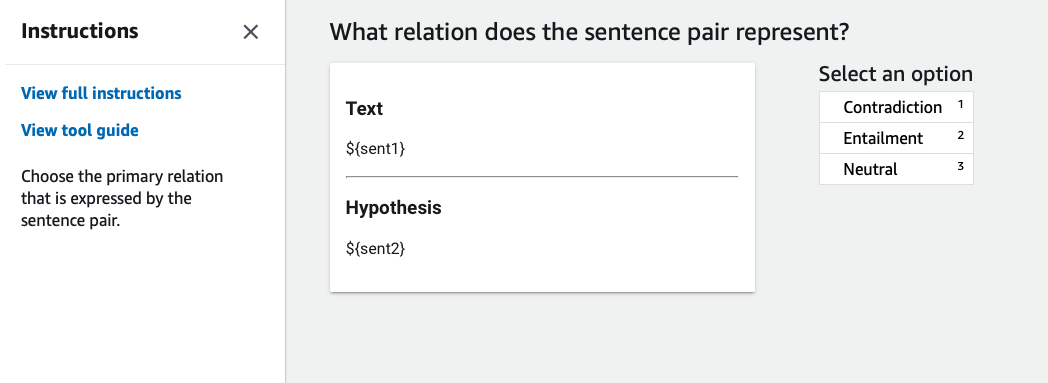
\includegraphics[width=300px]{images/amt-02.png}
  \caption{Entailment Annotation}
  \label{fig:entailann}
\end{figure}
첫 번째로, Entailment Annotation(Figure \ref{fig:entailann})의 경우
Article에서 추출된 문장 Pair를 보여주고, Contradiction / Entailment / Neutral의
세 가지 관계 중 하나를 마크할 수 있도록 하였습니다.

화면 왼쪽의 \textit{View full instructions} 메뉴를 누르면
다음과 같이 선택지에 대한 detail이 표시되도록 하였습니다.

\noindent
\begin{center}
  \fbox{
  \begin{minipage}{0.8\linewidth}
  \textbf{Contradiction} the text contradicts hypothesis. \\
  \textbf{Entailment} the text entails hypothesis. \\
  \textbf{Neutral} the text does not entail nor contradict.
\end{minipage}}
\end{center}

\begin{figure}[!htbp]
  \centering
  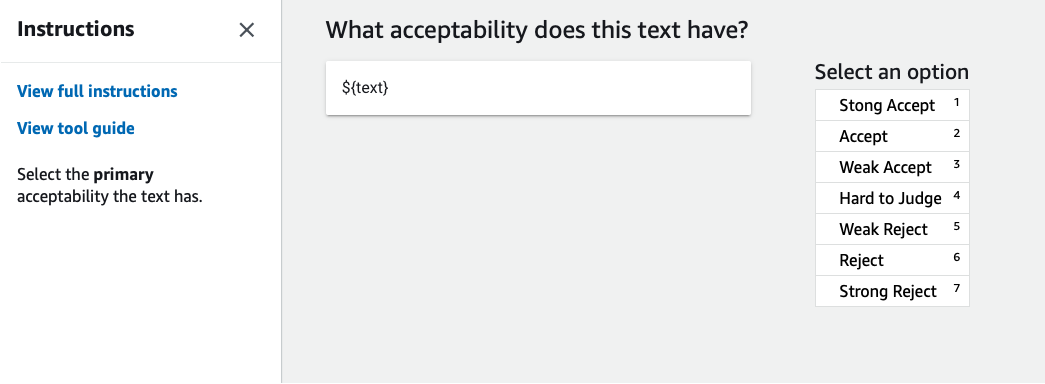
\includegraphics[width=300px]{images/amt-01.png}
  \caption{Entailment Annotation}
  \label{fig:acceptann}
\end{figure}

Acceptability Annotation(Figure \ref{fig:acceptann})도
거의 동일한 형식을 사용하였습니다.
\textit{View full instruction} 메뉴에 표시되는 텍스트는 다음과 같습니다.
기존 설문에 사용하던 Acceptability에 대한 설명을 그대로 사용하였습니다.

\noindent
\begin{center}
  \fbox{
  \begin{minipage}{0.8\linewidth}
  \textbf{Strong Accept}: I accept the information given by the sentence to be true. I have sound and cogent arguments to justify my acceptance. I am sure that I can effectively convince others that my judgement is reasonable. \\
  \textbf{Accept}: I accept the information given by the sentence to be true. I have some arguments to justify my acceptance. But I am not sure whether I can effectively convince others that my judgement is reasonable. \\
  \textbf{Weak Accept}: I accept the information given by the sentence to be true. I don’t have arguments justifying my acceptance. Still, I will accept it rather than reject it. \\
  \textbf{Hard to Judge}: It is hard to judge whether I should accept or reject the information given by the sentence to be true. \\
  \textbf{Weak Reject}: I reject the information given by the sentence to be true. I don’t have arguments for the rejection. Still, I will reject it rather than accept it. \\
  \textbf{Reject}: I reject the information given by the sentence to be true, and I have arguments for the rejection. But I am not sure whether I can effectively convince others that my judgement is reasonable. \\
  \textbf{Strong Reject}: I reject the information given by the sentence to be true. I have sound and cogent arguments for the rejection. I am sure that I can effectively convince others that my judgement is reasonable.
\end{minipage}}
\end{center}

\section{데이터}
설문에 사용될 데이터는 다음(Figure \ref{fig:data})과 같습니다.
\begin{figure}[!htbp]
  \centering
  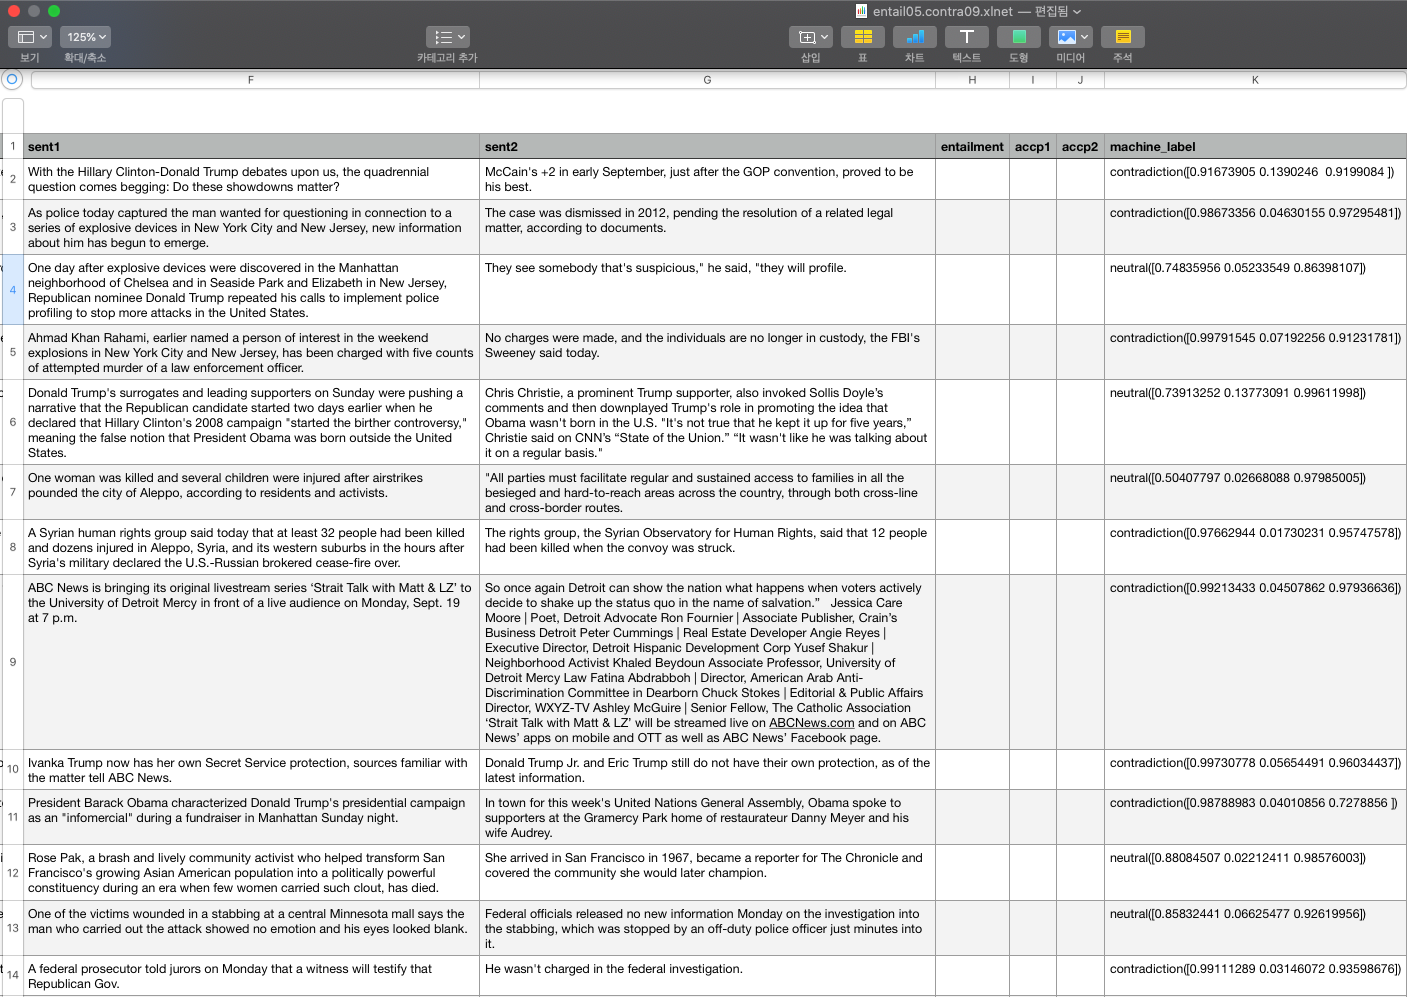
\includegraphics[width=400px]{images/amt-03.png}
  \caption{Data}
  \label{fig:data}
\end{figure}
\textbf{sent1} 컬럼은 news article의 첫 문장,
\textbf{sent2} 컬럼은 multiNLI corpus에 대해 pretrain된 모델로 추출한 문장입니다.
모델이 두 문장 사이의 관계를 추측한 결과는 \textbf{machine\_label} 컬럼에 기재되어 있습니다.

현재 여러 파라미터 조정을 거쳐, \textbf{machine\_label} 컬럼 기준
contradiction 764개, entailment 133개, neutral 707개의 문장 pair를 만들었습니다.
모델이 같은 기사 내에서 entailment 관계에 있다고 판단하는 문장의 수가 꽤 적어 machine label의 비율이 잘 맞지 않는 것과,
모델이 판단한 relation과 사람의 직관으로 판단한 relation이 다른 경우가 꽤 있는 것이 데이터셋의 문제가 될 수 있을 것 같습니다.

예를 들어, 아래의 예시 문장은 pretrained 모델이 contradiction으로 판단하였으나,
직관적으로 판단하였을 때는 contradiction과는 거리가 멂을 확인할 수 있습니다.
이런 경우 데이터셋의 설문 결과의 불균형이 일어날 수 있을 것으로 생각되는데, 더 좋은 문장 추출 방법을 생각 및 검색하는 중입니다.
\noindent
\begin{center}
  \fbox{
  \begin{minipage}{0.8\linewidth}
  \textbf{Text}: One woman was killed and several children were injured after airstrikes pounded the city of Aleppo, according to residents and activists. \\
  \textbf{Hypothesis}: ``They had dust in their lungs and we gave them oxygen.''
\end{minipage}}
\end{center}

또한, acceptability annotation의 경우 문장에 pronoun이 포함되는 것이 결과에 영향을 줄 수 있을 것으로 생각됩니다.
따라서, 해당 문장이 포함된 기사와 함께 문장을 하이라이트하여 보여줆으로써 문제를 해결하는 방안을 생각하고 있습니다.


\end{document}